% DESCRIÇÃO DA IMPLEMENTAÇÃO-------------------------------------------------------------------

\chapter{DESCRIÇÃO DA IMPLEMENTAÇÃO}
\label{chap:descricao_da_implementacao}

% ADAPTIVE DSD-------------------------------------------------------------------
\section{\adaptive{}}
\label{sec:adaptiveDSD}

O \adaptive (\textit{Adaptive Distributed System-Level Diagnosis}) é um algoritmo para diagnóstico em redes completamente conectadas. Onde seu funcionamento é, ao mesmo tempo 
adaptativo e distribuído. Foi desenvolvido para que cada máquina que possua o algoritmo em execução possa realizar o teste e também ser testada por outras máquinas na rede.
É caracterizado como adaptativo por não depender e nem restrigir o número de máquinas na rede, necessitando, no mínimo uma máquina para o teste. Para a execução dos testes, não é levado
em consideração falhas na rede, pois o objetivo deste algoritmo é, testar o processamento ou funcionamento específico de um processo na máquina.

\subsection{Funcionamento}
\label{sub:adaptiveDSD_Funcionamento}
O algoritmo possui duas listas, que possuem de tamanho o número de máquinas conectadas à rede, as listas são: o vetor TESTED\_UP, que irá guardar na posição da máquina atual, 
o índice da máquina testada que possui funcionamento normal; o vetor STATE, que armazena o estado das máquinas, tendo inicialmente o valor FALHO para todas e, caso uma máquina tenha seu 
funcionamento correto confirmado, esta receberá o valor NORMAL no vetor. A cada rodada os vetores são atualizados e enviados às outras máquinas na rede.

Na primeira rodada, uma máquina irá iniciar o teste seguindo a lista de máquina existentes e disponíveis na rede. Esta máquina irá percorrer a
lista de máquinas e fará uma requisição de teste à próxima máquina da lista. No caso da máquina à ser testada retornar uma resposta de funcionamento correto, a máquina que está realizando o 
teste atualiza os dados e envia à máquina testada, que por sua vez irá executar o mesmo processo com a máquina seguinte, até que todas as máquinas tenham sido testadas. Por outro lado, se 
a máquina testada retornar algum erro, será marcada como falha, e a máquina que está testando irá testar a próxima máquina da lista, até encontrar outro máquina com funcionamento normal 
ou até que a lista de máquinas disponíveis acabe.

A segunda rodada será para atualizar as informações de todas as máquinas na rede sobre o estado de funcionamento de cada máquina. Inicialmente a primeira máquina com funcionamento normal 
irá verificar na lista de máquinas, qual a próxima máquina funcionando e irá enviar os dados da rede. Ao receber os dados da rede, a máquina receptora irá prosseguir com a distrbuição 
de informações.

\subsection{Algoritmo}
\label{sub:adaptiveDSD_Algoritmo}
O algoritmo \adaptive inicia sua execução criando uma conexão em uma porta por um \textit{socket} e fica escutando esta porta, até que uma conexão seja estabelecida por outra máquina.
Ao final de toda requisição realizada por outro máquina, o algoritmo volta a escutar e aguardar uma nova conexão por \textit{socket} com a porta.

\vspace*{1cm}
\begin{python}
    tcp = socket.socket(socket.AF_INET, socket.SOCK_STREAM)
    tupla = (ip_host, int(porta_host))
    tcp.bind(tupla)
    tcp.listen(1)

    conexao, cliente = tcp.accept() 
    ReceberRequisicao(conexao)
\end{python}
\vspace*{1cm}

O método \textbf{ReceberRequisicao} direciona para o fluxo requisitado pela máquina que está conectando com a máquina atual. As seguintes mensagens podem ser enviadas para realizar determinadas ações:

\vspace*{1cm}
\begin{enumerate}
    \item \textbf{'start'}: mensagem enviada pelo gerenciador para realizar uma verificação das máquinas. A máquina será considerada a primeira da lista (posição 0) e terá o estado NORMAL. Ao receber esta mensagem,
    irá executar o método IniciarTeste.
    \item \textbf{'check'}: mensagem enviada pela máquina que está realizando o teste no momento. Ao receber esta mensagem a máquina atual irá realizar uma verificação de funcionamento e, 
    irá retornar se possui falha ou não.
    \item \textbf{'keepTest'}: mensagem enviada pela máquina que está realizando o teste caso a máquina atual esteja com funcionamento NORMAL. Informa a máquina atual para dar continuidade ao teste de funcionamento.
    \item \textbf{'keepInfo'}: mensagem enviada por uma máquina na lista de máquinas com status NORMAL. Informa a máquina atual para manter as informações do teste realizado e prosseguir com a distribução da informação.
    \item \textbf{'info'}: mensagem enviada pelo gerenciador para receber as informações do ultimo teste. A máquina atual irá retornar ao gerenciador o status de cada máquina da rede.
  \end{enumerate}

\vspace*{1cm}
\begin{python}
    msg = ReceberResposta(conexao)
    if msg == "start":
        IniciarTeste(conexao)
    elif msg == "check":
        RealizarVerificacao(conexao)
    elif msg == "keepTest":
        ContinuarTeste(conexao)
    elif msg == "keepInfo":
        ManterInformacao(conexao)
    elif msg == "info":
        RetornaInformacao(conexao, False)
\end{python}
\vspace*{1cm}

O método \textbf{IniciarTeste} inicia recebendo do gerenciador uma lista das máquinas, contendo o IP e porta, para conexão. Cria as listas TESTE\_UP e STATE e inicia o teste.

O método \textbf{TestarMaquina} percorre a lista de máquinas, executa o método \textbf{CriarConexao} para criar a conexão com a máquina a ser testada e envia a mensagem 'check'. Caso 
a máquina testada retornar a confirmação de funcionamento, a máquina atual procede em enviar as informações existentes à máquina testada, primeiramente enviando a mensagem 'keepTest' para informar a outra máquina 
a dar continuidade no teste. Caso a máquina testada retornar erro, esta será marcada com um 'X' no vetor TESTED\_UP e como 'FALHO' no vetor STATE.
Ao chegar na última máquina da lista, o método \textbf{DistribuirInformacao} é executado.

\vspace*{1cm}
\begin{python}
    maquina = CriarConexao(host, porta)
    msg = EnviarInformacao(maquina, "check")
    if msg == "OK":
        maquina = CriarConexao(host, porta)
        EnviarInformacao(maquina, "keepTest")
        EnviarInformacao(maquina, json_maquinas)
        EnviarInformacao(maquina, json_tested)
        EnviarInformacao(maquina, json_state)
        break
    else:
        tested_up[index] = "X"
        state[index] = "FALHO"
        index = index + 1
\end{python}
\vspace*{1cm}

O método \textbf{ContinuarTeste} recebe as informações coletadas até o momento no teste, enviando uma confirmação a cada envio. Após isto, uma verificação é realizada para direcionar 
o teste para próxima máquina da lista, ou para iniciar a distrbuição das informações, caso não haja mais máquinas não testadas na rede.

O método \textbf{ManterInformacao} recebe as informações do teste finalizado, enviando uma confirmação a cada envio. Por fim, a máquina envia estas informações à próxima máquina com status 
'NORMAL'.

O método \textbf{RetornaInformacao} retorna as informações do teste. Caso o parâmetro \textbf{verificacao} seja verdadeiro, ao enviar uma informação, a máquina irá esperar por uma resposta 
de confirmação, se não, irá apenas enviar as informações, sem esperar por uma resposta de confirmação.




% API-------------------------------------------------------------------
\section{\textit{API}}
\label{sec:api}









% Frontend-------------------------------------------------------------------
\section{\textit{Frontend}}
\label{sec:frontend}

Desde o princípio do projeto, os integrantes do grupo optaram por modulizar a solução, encarregando cada parte com sua respectiva função, tal como: o \adaptive{} (subcapítulo \ref{sec:adaptiveDSD}) seria responsável apenas por detectar falhas na rede; a \textit{API} (subcapítulo \ref{sec:api}) faria a comunição entre os módulos; o \textit{frontend} (subcapítulo atual) seria responsável por apresentar ao usuário uma tela simples e intuitiva e a \textit{PWA} (subcapítulo \ref{sec:pwa}) é um complemento ao projeto, que servirá para dar mais mobilidade ao utilizador da plataforma.

Esta decisão possibilitou que o \textit{frontend} fosse criado com foco total em proporcionar a melhor experiência possível para o usuário, consumindo e exibindo todas informações disponibilizadas pela \textit{API}. Tendo em vista que o \adaptive{}será executado em intervalos de tempo, as páginas precisariam repassar esse dinamismo ao usuário e, buscando obter caraterística, toda a parte visual do projeto foi construída utilizando \textit{React} - uma biblioteca JavaScript focada na criação de interfaces de usuário, desenvolvida pelo Facebook.


\subsection{O Sistema}
\label{sec:o_sistema}

Essa biblioteca realmente atendeu às expectativas e permitiu que as duas principais telas do sistema fossem criadas realmente conforme o pretendido. A primeira, que pode ser visualizada na figura \ref{fig:landing_page}, serve simplesmente como uma tela de boas-vindas ao usuário, na qual ele poderá ler um breve resumo do que é a plataforma, entender em quais pontos ela pode ser útil e ver quem são as membros da equipe que criou o projeto.

\begin{figure}[H]
    \centering
    \caption{\textit{Landing Page}}
    \frame{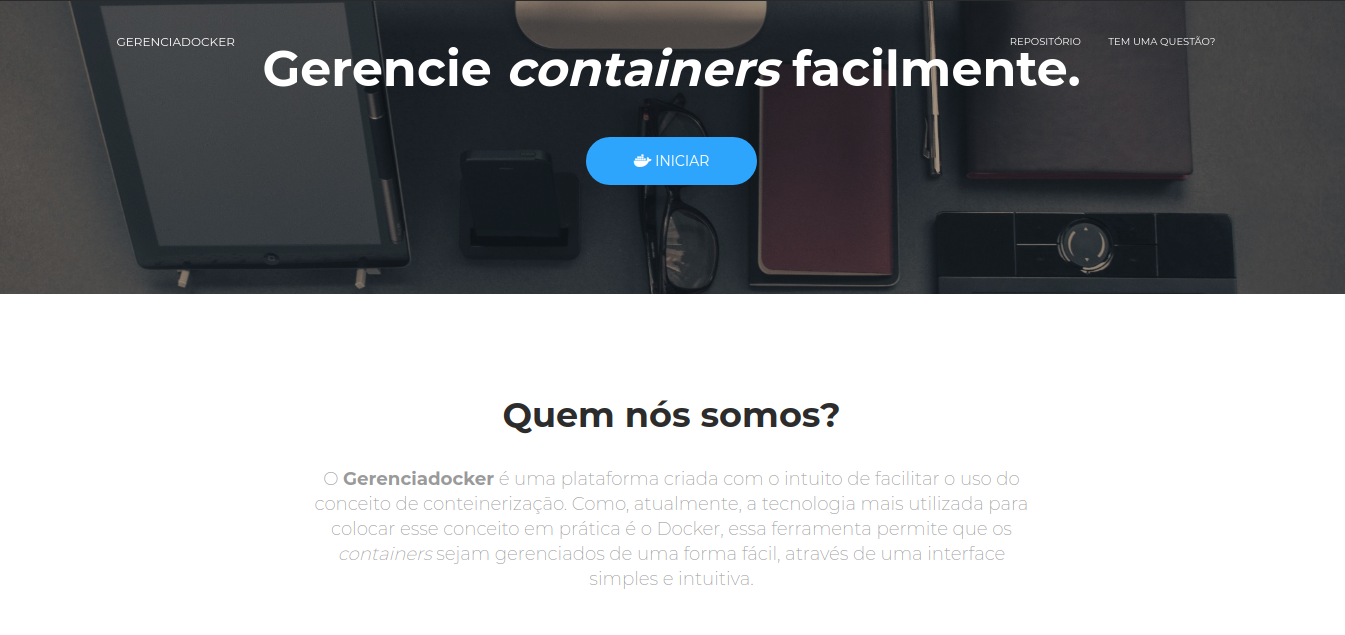
\includegraphics[width=1.0\textwidth]{./content/textuais/imagens/landing-page.png}}
    \label{fig:landing_page}
\end{figure}

Já a segunda, que é a tela de demonstração, é o local mais importante do sistema e pode ser acessado através do botão \aspas{Iniciar} exibido na figura \ref{fig:landing_page}. É nesse ambiente que o usuário criará sua \dockerNetwork{} e visualizará o estado atual de cada um dos \containers{} que a compõe. Além disso, também é possível interagir com cada \conteiner{} individualmente e utilizar opções como \aspas{Pausar}, \aspas{Retomar} ou \aspas{Excluir}, tal como pode ser visualizado na figura 3.

{\huge TELA DE DEMONSTRAÇÃO AQUI}








% PWA-------------------------------------------------------------------
\section{PWA}
\label{sec:pwa}

Os \textit{Progressive Web Apps}, que recentemente vem ganhando bastante popularidade e adeptos, podem ser definidos como \cite{Souza19} \aspas{uma aplicação \web{} com tecnologias que permitem termos a experiência de uso muito próxima da oferecida pelos \textit{mobile apps}}. Isso quer dizer, basicamente, que ao acessar um \textit{site}, o usuário terá a opção de adicionar um \aspas{atalho} para este no seu celular.

Porém, ao abrir esse atalho, a experiência para o utilizador será de estar utilizando um aplicativo nativo, como se tivesse \aspas{instalado o \textit{site}} em seu dispositivo. Isso porque ele não verá uma barra exibindo a \textit{URL} que está sendo acessada e, além disso, funções nativas do celular - como acesso à câmera, geolocalização, aos contatos e \textit{push notifications} - estarão em pleno funcionamento. Esse tipo de solução tem sido testada e utilizada por grandes empresas como Uber, Twitter e Facebook, por exemplo, em virtude de algumas vantagens que ela apresenta sobre os \textit{apps} nativos, principalmente em dois pontos: custos e engajamento do cliente.


Primeiramente, no quesito despesas, utilizar um \textit{PWA} permite que, com poucas alterações no site da empresa, ela disponibilize um \aspas{aplicativo} - o que economiza tempo de desenvolvimento e, consequentemente, dinheiro. Em segundo lugar, geralmente os \textit{PWAs} são mais rápidos, ocupam menos espaço de armazenamento no dispositivo e, em casos reais, ficou comprovado que a facilidade em obter esse \textit{app} gera mais conversão de clientes, conforme \cite{Souza19} \aspas{o Flipkart que é o maior e-commerce da Índia, eles decidiram fazer uma experiência mobile através de uma PWA e aumentaram a sua conversão em 70\%}.

Para resumir, sempre que deseja-se criar uma experiência agradável para o usuário, de forma rápida e com poucos custos, não sendo necessário implementar funcionalidades demasiadamente robustas, um \textit{PWA} é a melhor opção. No caso desse projeto, portanto, que se enquadra perfeitamente nessas características, o grupo considerou essa como sendo a tecnologia ideal para criarmos um aplicativo para este projeto.


\subsection{O Aplicativo}
\label{subsec:o_aplicativo}

Para tornar a solução ainda mais completa e próxima das necessidades do usuário, o grupo decidiu fazer um \textit{app} simples (utilizando a tecnologia citada no subcapítulo \ref{sec:pwa}) que irá listar todas as ocorrências de falhas nos \containers{}, além de disparar uma \textit{push notification} na tela do usuário. O objetivo principal deste aplicativo é servir como uma fonte de consulta para o usuário responsável pelo funcionamento da rede de \containers{}.

Isso porque, em virtude de relacionar-se com diversas variáveis (velocidade da rede, infraestrutura, tamanho das equipes, entre outras), é possível que esse tipo de rede apresente pequenas falhas com o decorrer do tempo. Como é de conhecimento de todos, o profissional moderno precisa, além de realizar várias tarefas em paralelo, contar com uma certa mobilidade e, portanto, não seria agradável que um colaborador precisasse monitorar a tela do sistema em tempo integral para identificar quando ocorresse um problema.

Em razão disso, era necessário chamar a atenção dos responsáveis por manter a rede funcionando de alguma forma. Analisando as tecnologias disponíveis nos dias de hoje, chegou-se ao consenso que uma notificação no celular é, provavelmente, um dos melhores meios de chamar a atenção de alguém. Na imagem abaixo, é possível visualizar a interface da versão final do aplicativo:

{\huge IMAGEM DA PWA AQUI}